各入射方向における測線で得られた波形データから群速度$\left<c_g\right>,\bar c_g$と
相互相関速度$\left<c_{cor}\right>, \bar c_{cor}$を計算した.その結果を
図\ref{fig:fig12}に示す.
この図は横軸が入射方向を,縦軸が音速値(km/s)を示している.
音速値は,概ね2.7(km/sec)から3.15(km/sec)の範囲にあり,主として表面波からなる
波動が観測されていることが分かる.この中で,最も方向による変化が大きいのは
平均群速度$\left<c_g\right>$で,$\theta=150$度と330度の方向で極大,
$\theta=30,240$度の方向で極小となっており,明確に音響異方性を示している.
一方,平均波形$\left<a \right>(t)$から求めた群速度$\bar c_g$の伝播方向による変動は
0.1(km/sec)と小さく,波形の平均化により速度の異方性が弱められることがわかる.
また,相互相関速度$\left<c_{cor}\right>$と$\bar{c}_{cor}$の挙動は,$\bar c_g$の挙動と
よく似ている.相互相関関数の計算では,参照波形として用いた入射波波形と類似した波形部分から到達時間を検出する.
そのため,最もよく位相が揃った波動が到達する時刻が得られるものの,観測点毎の速度変動が反映されにくいと考えられる.
以上のことから,音響異方性の評価には,局所的な群速度の平均$\left<c_g\right>$を見ることが
よいと言える.
%--------------------
\begin{figure}[h]
	\begin{center}
	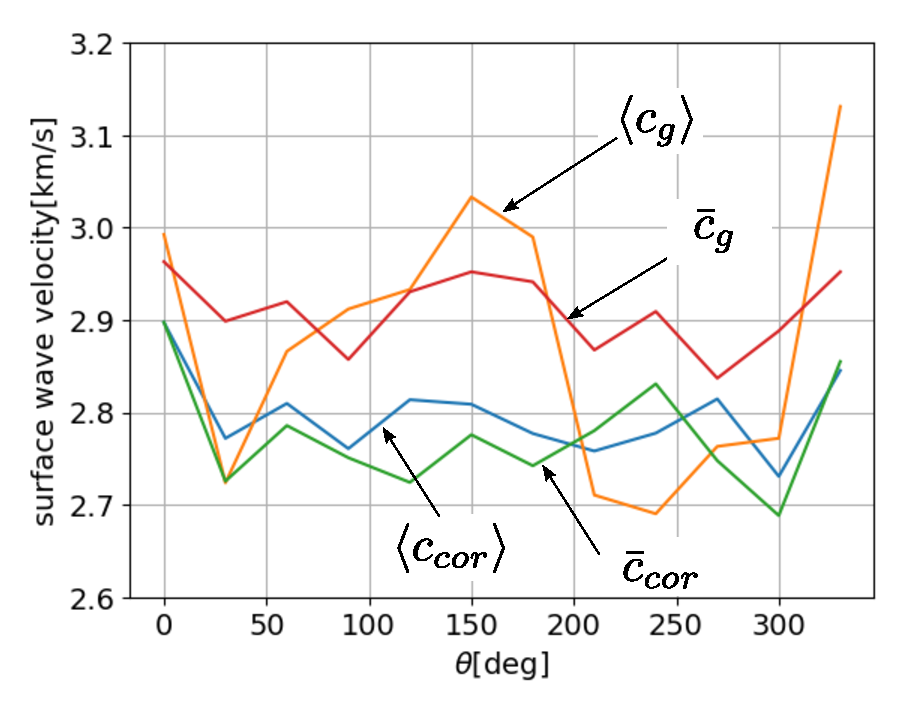
\includegraphics[width=0.8\linewidth]{Figs/fig12.eps} 
	\end{center}
	\caption{
		入射方向による群速度と相互相関速度の変化.
	} 
	\label{fig:fig12}
\end{figure}
%--------------------

ここで,入射方向毎に得られた平均波形$\left<a\right>(t)$を一覧すると,
図\ref{fig:fig11_1}のようになっている.
これら時刻歴波形の振幅はLDV出力の電圧値(mV)を表し,大小関係を波形相互に
比較でき,平均波形の最大振幅は明らかに方向によって変化している.そこで,
平均波形の最大振幅max$\left\{ \left< a \right>\right\}$と,
最大振幅の平均$\left< {\rm max}\left\{ a \right\} \right>$
が入射方向によってどのように変化するかを調べると,
図\ref{fig:fig14}のようになる.
この結果を図\ref{fig:fig12}と比べると,最大振幅の平均
$\left<{\rm max}\left\{a\right\}\right>$
は,$\left<c_g\right>$を上下に反転させたような形となり,強い異方性を
示すことが分かる.これは,群速度の速い方向で振幅が「小さく,
遅い方向で振幅が大きくなることを意味する.群速度と振幅値がこのような
相関を示すことは,岩石供試体の見かけの剛性が30度と240度方向で小さく,
150度と0度方向で大きくなるためと考えれば矛盾がない.
なお,平均波形の最大振幅max$\left\{\left<a\right>\right\}$は
最大振幅の平均よりも変動が若干小さい.これは,
波動到達時間の変動を考慮せずに最大値の平均をとる方が,
音響異方性をより敏感に反映した結果が得られることを意味する.
%--------------------
\begin{figure}[h]
	\begin{center}
	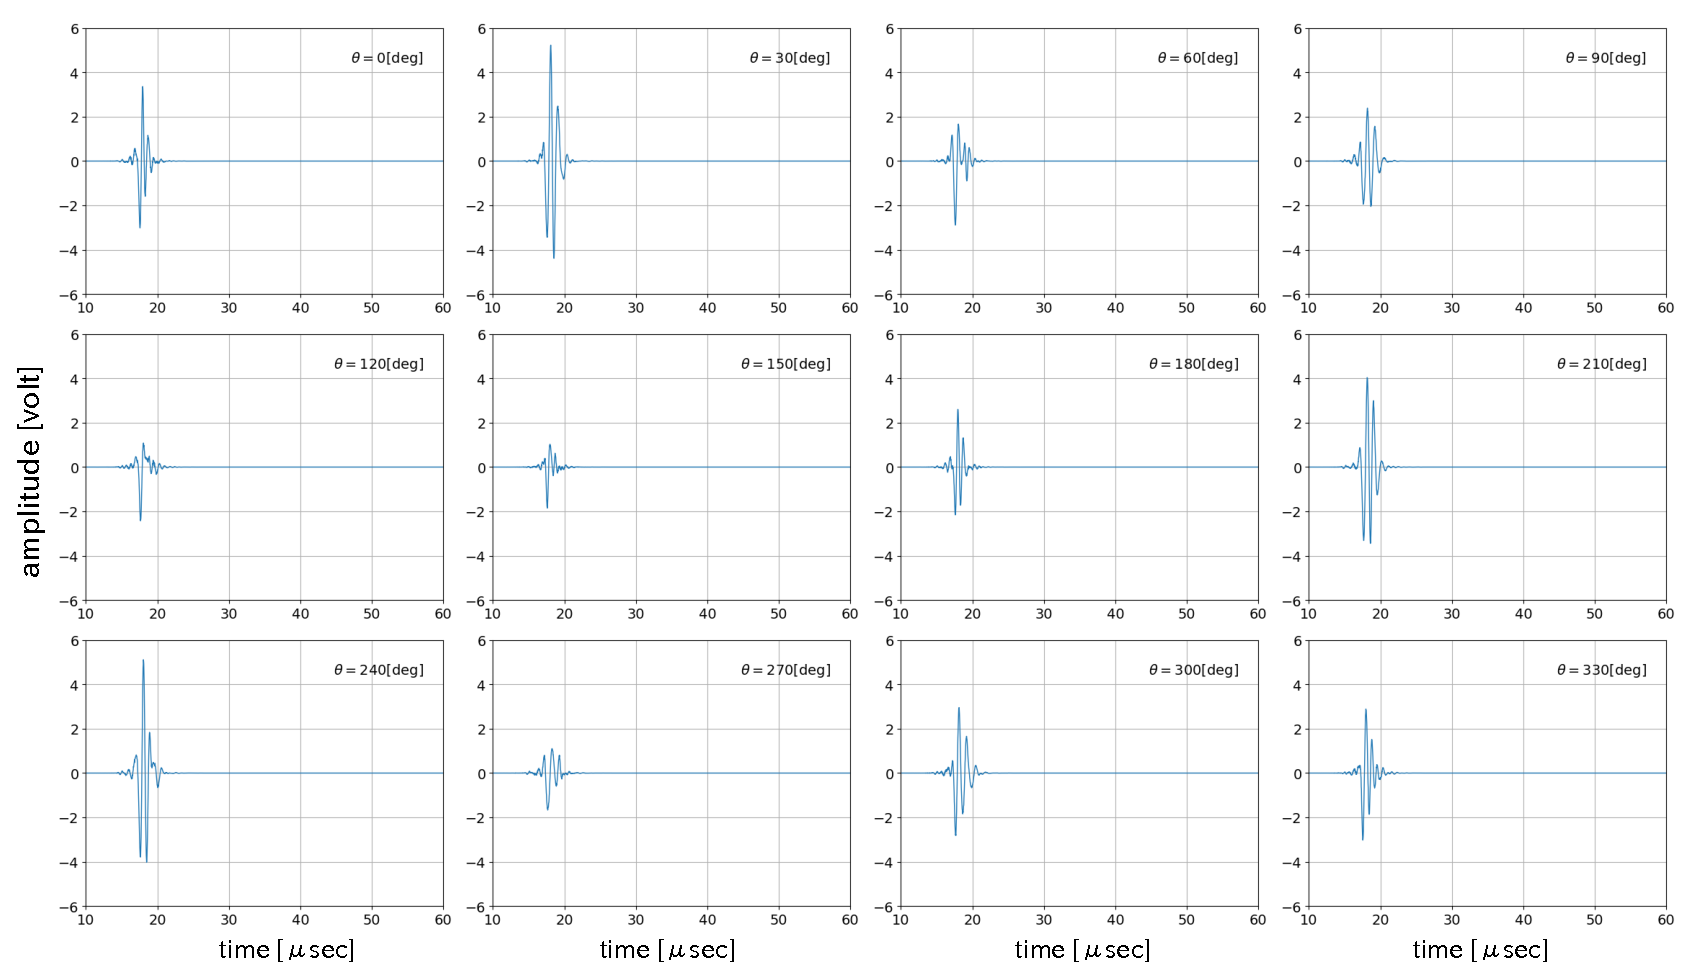
\includegraphics[width=1.0\linewidth]{Figs/fig11_1.eps} 
	\end{center}
	\caption{
		入射方向毎に得られた平均波形の時刻歴.
	} 
	\label{fig:fig11_1}
\end{figure}
%--------------------
\begin{figure}[h]
	\begin{center}
	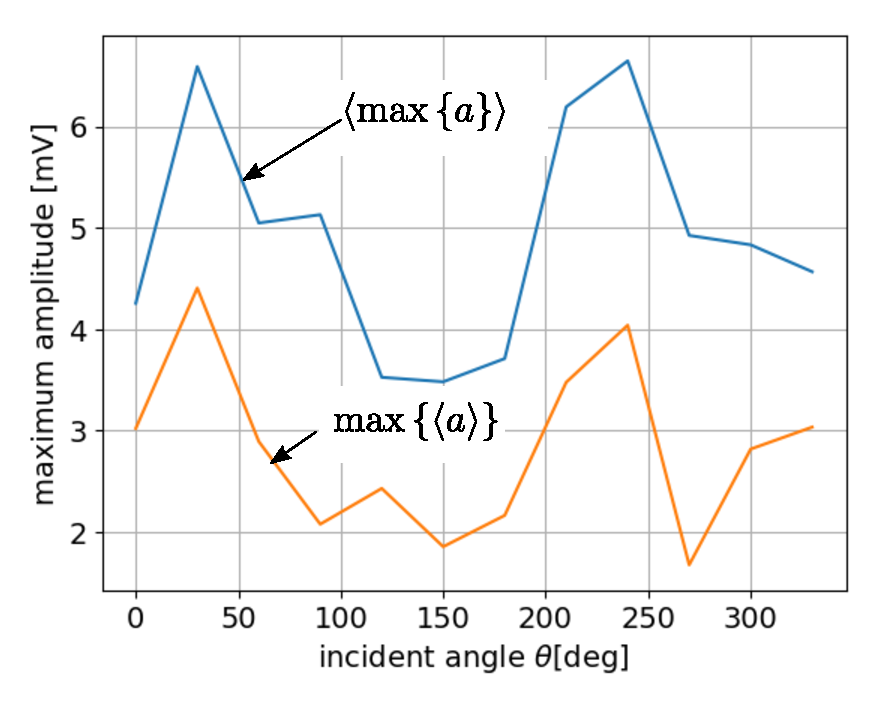
\includegraphics[width=0.8\linewidth]{Figs/fig14.eps} 
	\end{center}
	\caption{
		入射方向による最大振幅値の変化.
	} 
	\label{fig:fig14}
\end{figure}
最後に,平均波形の周波数スペクトル
\begin{equation}
	\left< A \right> (\omega) = \int \left<a\right>(t)e^{-i\omega t}dt
	\label{eqn:ave_A}
\end{equation}
を,入射方向毎に計算した結果を図\ref{fig:fig11_2}に示す.
これらの結果を見ると,周波数帯域はいずれの方向でも3MHz程度までとなっており,
その点に大きな違いは無い.一方,ピーク周波数には明らかなばらつきがあることに
気付く.そこで,平均波形のピーク周波数argmax$\left< A \right>$と,
個々の観測波形に対するピーク周波数の平均$\left< {\rm argmax }\left\{ A \right\}\right>$を求め,
角度との関係を示せば,図\ref{fig:fig13}のようになる.この図より,
ピーク周波数の平均$\left< {\rm argmax }\left\{ A \right\}\right>$は
$\left< c_g\right>$と似た傾向を示すことが分かる.具体的には,
群速度平均が大きな方向ではピーク周波数平均が高く,群速度平均が小さな方向では,
ピーク周波数平均は低くなっている.
これは,見かけの剛性が高い方が高周波の波を伝えやすく,みかけの剛性が低い方が
高周波成分を伝えにくいことを意味する.ここで,見かけの剛性と周波数が相関することは,
剛性の変化がマイクロクラックに起因したものであることを意味する.
なぜなら,線形弾性体では剛性の大小は振幅や音速に影響するが,周波数応答には
関与せず,剛性の周波数依存性は,界面の接触や滑りによってのみ生じるためである.
従って,ここで示した音響異方性に関する結果は,弾性波を使ったき裂評価において有用な
情報であると考えることができる.
なお,ピーク周波数の平均が,平均波形のピーク周波数よりも変動が小さい理由は
平均最大振幅と平均波形の最大振幅の大小に関する理由と同様である.
%--------------------
\begin{figure}[h]
	\begin{center}
	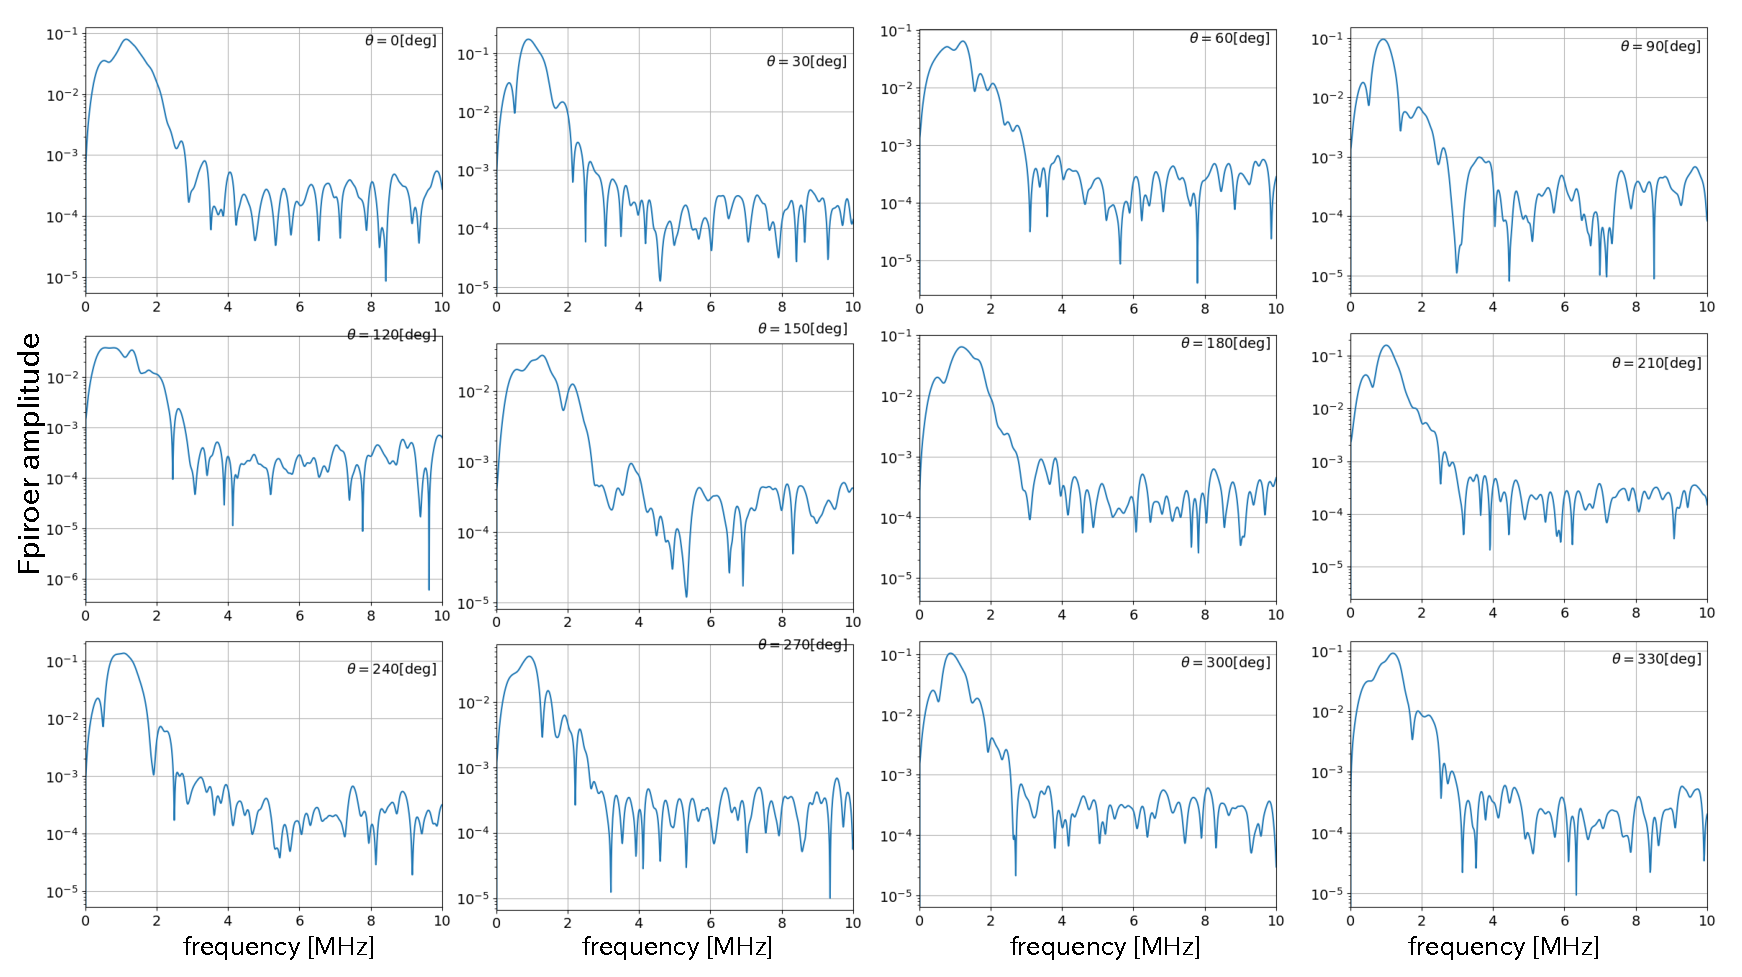
\includegraphics[width=1.0\linewidth]{Figs/fig11_2.eps} 
	\end{center}
	\caption{
		入射方向毎に得られた平均波形の周波数スペクトル.
	} 
	\label{fig:fig11_2}
\end{figure}
\begin{figure}[h]
	\begin{center}
	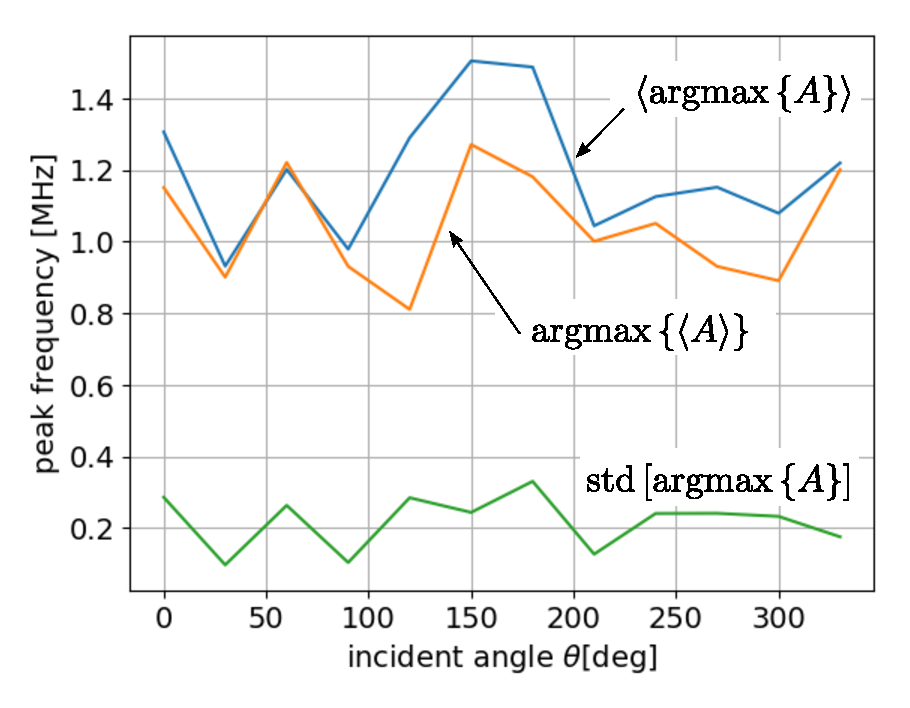
\includegraphics[width=0.8\linewidth]{Figs/fig13.eps} 
	\end{center}
	\caption{
		入射方向によるピーク周波の変化.
	} 
	\label{fig:fig13}
\end{figure}
%--------------------

